% American Journal of Physics -- Computational Physics section
%
% Build:  pdflatex manuscript && bibtex manuscript && pdflatex manuscript && pdflatex manuscript
%
% AJP reviews anonymously. Compiled directly, this file carries no names or
% affiliations and omits the acknowledgments, which is the version to upload at
% first submission. Compile manuscript_named.tex for the version with authors.
\newif\ifanon
\ifdefined\named\anonfalse\else\anontrue\fi

\documentclass[prb,preprint,amsmath,amssymb]{revtex4-2}
\usepackage{graphicx}
\usepackage{bm}
\usepackage[hidelinks]{hyperref}
\graphicspath{{../figures/}}
% Generated by code/analysis.py from data/summary.json. Do not edit by hand.
\newcommand{\secPerUnit}{0.319}
\newcommand{\lamBen}{0.299}
\newcommand{\lamBenEns}{0.296}
\newcommand{\nEns}{47}
\newcommand{\nChaotic}{44}
\newcommand{\nReg}{3}
\newcommand{\lamDir}{0.33}
\newcommand{\lamDirEarly}{0.28}
\newcommand{\lamDirLate}{0.33}
\newcommand{\lamDirOther}{0.329}
\newcommand{\slopeStep}{7.9}
\newcommand{\slopeStepSE}{0.4}
\newcommand{\slopeStepPred}{9.3}
\newcommand{\lamStep}{0.35}
\newcommand{\lamStepSE}{0.02}
\newcommand{\slopePrec}{1.99}
\newcommand{\slopePrecSE}{0.06}
\newcommand{\slopePrecPred}{2.32}
\newcommand{\lamPrec}{0.35}
\newcommand{\lamPrecSE}{0.01}
\newcommand{\gammaRound}{0.6}
\newcommand{\gammaLo}{0.3}
\newcommand{\gammaHi}{0.8}
\newcommand{\lamDirWin}{0.35}
\newcommand{\lamPrecCoarse}{0.31}
\newcommand{\lamPrecFine}{0.34}
\newcommand{\lamExcess}{18}
\newcommand{\TsingleFine}{30}
\newcommand{\collapseSpan}{8}
\newcommand{\collapse}{0.21}
\newcommand{\rkOrder}{4.000}
\newcommand{\ordEuler}{1.002}
\newcommand{\ordMid}{1.999}
\newcommand{\TEulerFine}{31}
\newcommand{\TRKcoarse}{43}
\newcommand{\TkEight}{79}
\newcommand{\TkEleven}{97}
\newcommand{\TBestDouble}{101}
\newcommand{\TBestDoubleSec}{32}
\newcommand{\kBestDouble}{11}
\newcommand{\TBestSingle}{53}
\newcommand{\TBestSingleSec}{17}
\newcommand{\kBestSingle}{7}
\newcommand{\kRatio}{64}
\newcommand{\TdoubleFine}{98}
\newcommand{\TdoubleKten}{92}
\newcommand{\dEexp}{10}
\newcommand{\costFactor}{2000}
\newcommand{\extraBits}{50}
\newcommand{\lamSI}{0.94}
\newcommand{\decadeSI}{10}
\newcommand{\bestRows}{24 (single) & $2^{-7}$ & 53 & 17 \\
32 & $2^{-7}$ & 66 & 21 \\
40 & $2^{-9}$ & 79 & 25 \\
53 (double) & $2^{-11}$ & 101 & 32 \\
64 (extended) & $2^{-15}$ & 124 & 40 \\}


\begin{document}

\title{How long is a simulated double pendulum right?\\
Step size, floating-point precision, and the Lyapunov exponent}

\ifanon
\else
\author{Luke Wang}
\author{Arjun Pemmasani}
\email{arjun.pemmasani@gmail.com}
\affiliation{Harvey Mudd College, Claremont, California 91711}
\fi

\date{\today}

\begin{abstract}
Students who simulate a chaotic system learn that nearby initial conditions
separate exponentially, but they seldom ask the corresponding question about the
simulation itself, which is perturbed at every step by truncation and by
roundoff. We describe a computational exercise that answers it. The double
pendulum is integrated with a fixed-step fourth-order Runge--Kutta method in
arbitrary-precision arithmetic, so that the step $h$ and the number of
significand bits $p$ can be varied independently, and we measure the time $T$
for which each computed trajectory agrees with a far more accurate reference.
The results follow a single formula in which the largest Lyapunov exponent
$\lambda$ is the only property of the pendulum that appears: halving $h$ extends
$T$ by $4\ln 2/\lambda$, and each additional bit extends it by $\ln 2/\lambda$,
until the other source of error takes over. The numerical error therefore
measures $\lambda$. The two values obtained this way, $\lamStep\pm\lamStepSE$ and
$\lamPrec\pm\lamPrecSE$ in natural units, match the growth rate of a deliberately
perturbed trajectory over the same interval and lie within 20\% of the long-time
exponent, \lamBen. In double precision no choice
of step keeps this pendulum accurate beyond about \TBestDouble\ natural time
units, roughly \TBestDoubleSec~s for rods one meter long, and the computational
work needed grows exponentially with $T$. Energy, meanwhile, remains conserved to
a part in $10^{\dEexp}$ long after the trajectory has become wrong. The
exercise needs about forty lines of code and turns numerical error from a
nuisance into a measuring instrument.
\end{abstract}

\maketitle

\section{Introduction}

The double pendulum is the standard classroom example of chaos in a mechanical
system, and this journal has treated it as one for thirty years. Shinbrot
\textit{et al.}\cite{shinbrot1992} released two nearly identical physical
pendulums together, watched them separate, and measured an exponential growth
rate of $7.5\pm1.5~\mathrm{s^{-1}}$. Levien and Tan\cite{levien1993} built a
double pendulum for the undergraduate laboratory and compared its motion with a
numerical model. More recently D'Alessio\cite{dalessio2023} combined analysis,
simulation and experiment and computed the full spectrum of Lyapunov exponents.
All three ask how the \emph{physical} system amplifies an uncertainty in its
initial state.

A simulation is subject to the same amplification, with one difference. Its
error is not confined to the initial condition. A small error is committed at
every step, from truncating the Taylor series of the solution and from rounding
each arithmetic result to a finite number of bits, and every one of those errors
is amplified from the moment it is made. A student who animates a double pendulum
for a minute therefore has no way of knowing whether the last forty seconds bear
any relation to the solution of the equations that were typed in. The checks
students usually reach for do not settle the matter. Energy can be conserved to
many digits by a trajectory that is entirely wrong, as we show in
Sec.~\ref{sec:energy}, and halving the step and seeing no visible change tests
only the interval over which nothing has yet gone wrong.

This paper describes an exercise that answers the question quantitatively. None
of the underlying facts is new. Lorenz\cite{lorenz1963} found sensitive dependence
by re-entering rounded numbers into a running computation;
Lighthill\cite{lighthill1986} gave the horizon of predictability its name; the
competition between truncation and roundoff is standard numerical
analysis;\cite{hairer1993} and the reliability of computed chaotic solutions has
been studied in the research literature on atmospheric models\cite{teixeira2007}
and with multiple-precision arithmetic.\cite{liao2009} What we have not found is
a treatment at the level of an undergraduate course in which the student
separates the two sources of error, measures each, and connects both to the
Lyapunov exponent. That is what is offered here. The exercise teaches five things:
\begin{enumerate}
\item The time for which a simulation of a chaotic system is accurate depends
only logarithmically on the error committed per step, so that large
improvements in the integrator buy modest extensions of that time.
\item Truncation error and roundoff error can be isolated from one another
cleanly once the precision of the arithmetic is a parameter of the program rather
than a property of the hardware.
\item Numerical error is itself a small perturbation, and its growth measures the
Lyapunov exponent as well as a deliberately perturbed initial condition does.
\item For a given floating-point format there is a best step, and a longest
accurate time that no step can improve upon.
\item Conservation of energy is not evidence that a chaotic trajectory is
correct.
\end{enumerate}

\section{Model and numerical method}

\subsection{Equations of motion}

Two point masses $m$ hang in series from a fixed pivot on massless rigid rods of
length $l$ and move in a vertical plane under gravity. With the angles
$\theta_1$ and $\theta_2$ measured from the downward vertical and time in units
of $\sqrt{l/g}$, the Lagrangian equations of motion contain no parameters:
\begin{align}
\ddot\theta_1 &= \frac{\omega_1^2\sin\Delta\cos\Delta+\sin\theta_2\cos\Delta
                +\omega_2^2\sin\Delta-2\sin\theta_1}{2-\cos^2\Delta},\label{eq:eom1}\\
\ddot\theta_2 &= \frac{-\omega_2^2\sin\Delta\cos\Delta
                +2\left(\sin\theta_1\cos\Delta-\omega_1^2\sin\Delta-\sin\theta_2\right)}
                {2-\cos^2\Delta},\label{eq:eom2}
\end{align}
where $\omega_i=\dot\theta_i$ and $\Delta=\theta_2-\theta_1$. The energy, in
units of $mgl$, is
\begin{equation}
E=\omega_1^2+\tfrac12\omega_2^2+\omega_1\omega_2\cos\Delta-2\cos\theta_1-\cos\theta_2 .
\label{eq:energy}
\end{equation}
Every run starts from rest with both rods horizontal,
$\theta_1=\theta_2=\pi/2$, for which $E=0$. One natural time unit is
\secPerUnit~s when $l=1$~m.

\subsection{Integrator and arithmetic}

We write Eqs.~(\ref{eq:eom1}) and (\ref{eq:eom2}) as a first-order system
$\dot{\bm y}=\bm f(\bm y)$ for $\bm y=(\theta_1,\theta_2,\omega_1,\omega_2)$ and
advance it with the classical fourth-order Runge--Kutta method (RK4) at a fixed
step $h$. A fixed step is essential to the exercise. An adaptive integrator
adjusts $h$ to hold its own estimate of the local error near a tolerance, which
hides the dependence we wish to expose.

All arithmetic is carried out by the MPFR library,\cite{fousse2007} which rounds
every operation correctly to a significand of $p$ bits, with $p$ chosen by the
program. We call it from Python through the \texttt{gmpy2} package; Julia's
built-in \texttt{BigFloat} type wraps the same library and serves equally well.
The values $p=24$, 53, 64 and 113 reproduce the significand widths of IEEE
single, double, extended and quadruple precision,\cite{goldberg1991} and $p=237$,
that of the 256-bit format, stands in for exact arithmetic: its rounding unit is
$2^{-237}\approx10^{-71}$.

Steps are powers of two, $h=2^{-k}$. A power of two is represented exactly at
every precision, so that lowering $p$ changes the arithmetic and nothing else. A
decimal step such as $10^{-4}$ would be rounded differently at each precision,
and runs intended to differ only in their arithmetic would also be integrating
with slightly different steps.

\subsection{Reference solution and measure of error}

The error of a run is measured by the distance $d(t)$ between its lower bob and
that of a reference run, in units of $l$. Since both bobs lie within $2l$ of the
pivot, $d$ saturates near 4 once two runs have nothing to do with each other. We
define the \emph{horizon} $T$ of a run as the first time at which
$d\ge10^{-2}$, which is roughly when two superimposed animations become visibly
different.

No exact solution is available to serve as the reference, so the reference is
simply a much more accurate run, and the following argument says how far it can
be trusted. Let $e_a$ and $e_r$ be the true errors of a run and of the reference.
By the triangle inequality the measured separation satisfies
$|d-e_a|\le e_r$. All errors are amplified at the same rate, so the ratio
$e_r/e_a$ stays close to its initial value, which for two RK4 runs with steps
$2^{-k_r}$ and $2^{-k_a}$ is $2^{-4(k_r-k_a)}$. Against a reference with
$k_r=18$, the separation therefore gives the true error of a run with
$k_a\le16$ to better than one part in 250, for as long as the run itself is
accurate.

\subsection{Three experiments}

\emph{Truncation alone.} With $p=237$ we vary $k$ from 4 to 17 and compare each
run with the reference $k=18$. Roundoff is some fifty orders of magnitude below
the truncation error and plays no part.

\emph{Roundoff alone.} With $h$ fixed we vary $p$ from 11 to 128 and compare each
run with the run at $p=237$ \emph{and the same} $h$. Both runs iterate the same
discrete map, so the truncation error is common to them and cancels exactly.
What remains is the effect of rounding. This separation is the step that
hardware arithmetic does not allow, and it is the reason for using a
multiple-precision library.

\emph{Both together.} With $p=24$, 32, 40, 53 and 64 we vary $k$ and compare with
the reference of the first experiment. This is the situation of a student
working in ordinary single or double precision.

\section{The horizon of predictability}
\label{sec:theory}

Let $\bm e_n$ be the error after $n$ steps. One step maps it to
$\bm e_{n+1}=\mathsf J_n\bm e_n+\bm\tau_n+\bm\rho_n$, where $\mathsf J_n$ is the
Jacobian of the flow across the step, $\bm\tau_n=O(h^5)$ is the local truncation
error of RK4, and $\bm\rho_n=O(2^{-p})$ is the rounding error committed in the
step. Unrolling the recursion expresses the error at time $t$ as a sum over all
earlier steps of the error committed there, carried forward by the product of the
intervening Jacobians. In a chaotic system that product grows on average as
$e^{\lambda(t-t_j)}$, where $\lambda$ is the largest Lyapunov exponent. The
sum is then a geometric series dominated by its earliest terms, and
\begin{equation}
e(t)\approx\left(A\,h^{4}+B\,2^{-p}h^{-\gamma}\right)e^{\lambda t}.
\label{eq:error}
\end{equation}
The first term collects $1/h$ truncation errors of size $h^5$ per unit time. The
second collects $1/h$ rounding errors of size $2^{-p}$ per unit time, which add
like a random walk, giving $\gamma=\tfrac12$, if their signs are independent and
linearly, giving $\gamma=1$, if they are not.\cite{hairer2008} The constants $A$
and $B$ depend on the trajectory but not on $h$ or $p$.

Setting $e(T)=\epsilon$ for a tolerance $\epsilon$ gives the horizon,
\begin{equation}
T=\frac1\lambda\,\ln\frac{\epsilon}{A\,h^{4}+B\,2^{-p}h^{-\gamma}} .
\label{eq:horizon}
\end{equation}
Everything in the exercise follows from Eq.~(\ref{eq:horizon}). When truncation
dominates and $h=2^{-k}$,
\begin{equation}
T=T_A+\frac{4\ln2}{\lambda}\,k ,
\label{eq:Tk}
\end{equation}
so that each halving of the step extends the horizon by the fixed amount
$4\ln2/\lambda$, the factor 4 being the order of the method. When roundoff
dominates,
\begin{equation}
T=T_B+\frac{\ln2}{\lambda}\left(p-\gamma k\right) ,
\label{eq:Tp}
\end{equation}
so that each additional bit extends the horizon by $\ln2/\lambda$, while each
halving of the step now \emph{shortens} it. The two regimes meet where the two
terms of Eq.~(\ref{eq:error}) are equal, at
$k^\ast=[\,p+\log_2(A/B)]/(4+\gamma)$, and the horizon there,
\begin{equation}
T_{\max}(p)\approx\mathrm{const}+\frac{\ln2}{\lambda}\,\frac{4p}{4+\gamma},
\label{eq:Tmax}
\end{equation}
is the longest attainable with $p$ bits and a fourth-order method. Both slopes
are properties of the pendulum alone, which is what allows the numerical error to
measure $\lambda$.

\section{Results}

\subsection{Step size}

Figure~\ref{fig:snap} shows what the experiment looks like. Three pendulums start
from identical states and are integrated with identical 237-bit arithmetic.
They differ only in $h$. For a long time they coincide to within the width of a
line, and then the one with the largest step departs, followed later by the
next. An animated version, in which the error curves are drawn alongside the
pendulums as they evolve, is included in the supplementary material and makes
the point to a class more quickly than any graph.

\begin{figure}
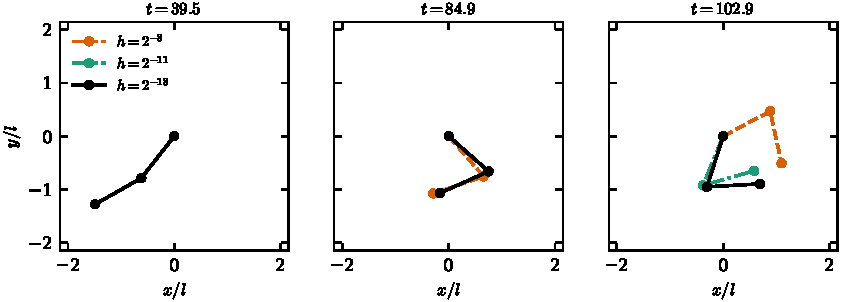
\includegraphics[width=\columnwidth]{fig1_snapshots}
\caption{Three double pendulums released from the same state and integrated with
the same 237-bit arithmetic, differing only in the step $h$. The run with
$h=2^{-8}$ leaves the others near $t=\TkEight$, and the run with $h=2^{-11}$ near
$t=\TkEleven$. Times are in units of $\sqrt{l/g}$.}
\label{fig:snap}
\end{figure}

Figure~\ref{fig:step}(a) shows $d(t)$ for a selection of steps. Each curve rises
through many orders of magnitude at the same average rate and then saturates. The curves are evenly spaced, and Fig.~\ref{fig:step}(b) shows why:
multiplied by $h^{-4}$ they collapse onto a single curve, to within
\collapse\ decades for every $h\le2^{-8}$ wherever none has saturated, and the
error at $t=10$ scales as $h^{\rkOrder}$. That curve
is the amplification factor of the trajectory itself. To confirm this we perturbed
$\theta_1(0)$ by $2^{-170}$, a perturbation small enough to remain in the linear
regime for the entire run, and plotted the resulting separation as the thin line
in Fig.~\ref{fig:step}(b). It follows the collapsed error curves through every
plateau and burst. The error of the integrator grows exactly as a perturbation of
the initial condition does, because it is one.

The growth is exponential only on average. The local rate fluctuates as the
pendulum passes through more and less unstable parts of its motion, and those
fluctuations are as much a part of the lesson as the mean.

\begin{figure}
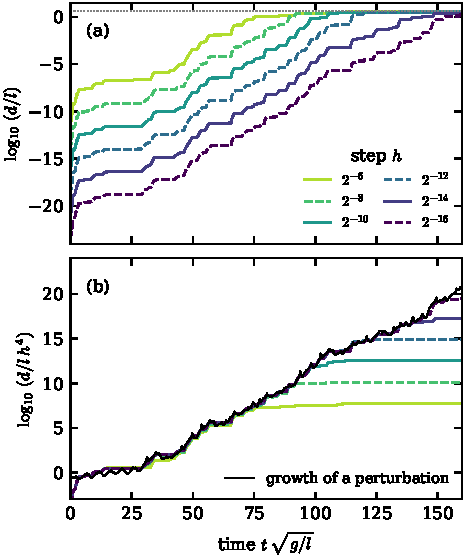
\includegraphics[width=\columnwidth]{fig2_step_sweep}
\caption{(a) Separation $d$ of the lower bob from that of the reference run
($h=2^{-18}$) for six values of the step, in 237-bit arithmetic; the running
maximum is shown. The dotted line marks the largest possible separation, $4l$.
(b) The same curves multiplied by $h^{-4}$ collapse. The thin black line is the
separation of two runs whose initial conditions differ by $2^{-170}$, shifted
vertically.}
\label{fig:step}
\end{figure}

The horizons are plotted against $k$ in Fig.~\ref{fig:hor}(a). A straight line
fitted for $7\le k\le16$ has slope $\slopeStep\pm\slopeStepSE$ time units per
halving of the step, and Eq.~(\ref{eq:Tk}) converts that to
$\lambda=\lamStep\pm\lamStepSE$. The scatter about the line is not noise. It is the
fluctuating local growth rate again: a horizon that falls just before a burst of
growth gains little from the next halving, and one that falls just after gains a
great deal. The gray staircase in Fig.~\ref{fig:hor}(a) makes this quantitative. It
is the horizon predicted for every $h$ from the measured growth of the $2^{-170}$
perturbation, with the single constant $A$ of Eq.~(\ref{eq:error}) taken from the
collapse, and it passes through the measured horizons step for step.

\begin{figure*}
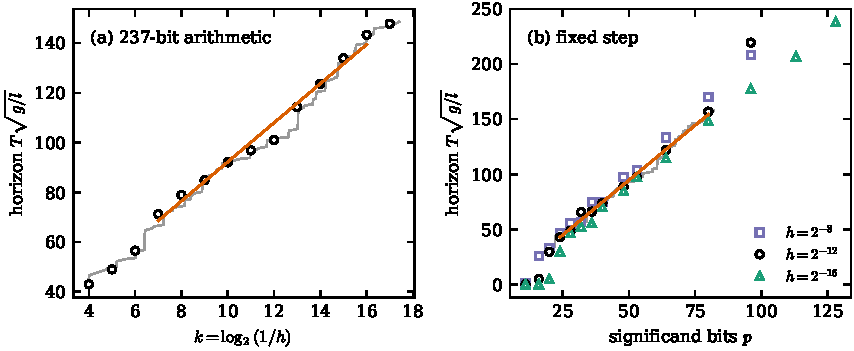
\includegraphics[width=\textwidth]{fig4_horizons}
\caption{Horizon $T$, the first time at which $d\ge10^{-2}$. (a) Against
$k=\log_2(1/h)$ in 237-bit arithmetic, where only truncation error is present.
(b) Against the number of significand bits $p$ at fixed step, where only
roundoff is present. The straight lines are least-squares fits whose slopes give
$\lambda$ through Eqs.~(\ref{eq:Tk}) and (\ref{eq:Tp}). The gray staircases are
the horizons predicted from the measured growth of a perturbation of the initial
condition.}
\label{fig:hor}
\end{figure*}

\subsection{Precision}

Figure~\ref{fig:prec} shows the second experiment for $h=2^{-12}$. The picture is
the same with $2^{-p}$ in place of $h^4$: evenly spaced curves, rising at a
common rate. The horizons in Fig.~\ref{fig:hor}(b) give a slope of
$\slopePrec\pm\slopePrecSE$ time units per bit and hence, from
Eq.~(\ref{eq:Tp}), $\lambda=\lamPrec\pm\lamPrecSE$. Changing the step by a factor
of 256 moves the line only slightly. Comparing the errors at fixed early times
for $h=2^{-8}$ and $2^{-16}$ gives $\gamma\approx\gammaRound$ in
Eq.~(\ref{eq:error}), with values between \gammaLo\ and \gammaHi\ for individual
precisions, which lies between the random-walk and the systematic limits.

\begin{figure}
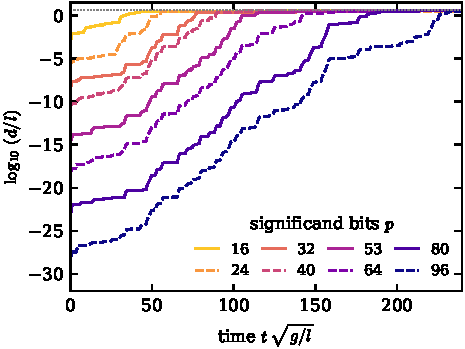
\includegraphics[width=\columnwidth]{fig3_precision_sweep}
\caption{Separation from the 237-bit run at the same step, $h=2^{-12}$, for
eight significand widths $p$. Truncation error is common to each pair of runs and
cancels, so the curves show the effect of roundoff alone.}
\label{fig:prec}
\end{figure}

The smallest precisions are excluded from the fit for a reason worth showing
students. With $p=11$ and $h=2^{-12}$ the pendulum \emph{never moves}. The first
increment to $\theta_1=\pi/2$ is smaller than half a unit in the last of eleven
bits, the sum rounds back to $\pi/2$, and the computed pendulum remains
horizontal forever. With the same eleven bits and $h=2^{-8}$ it falls. Here a
smaller step has not reduced the error but made it total, and no analysis
based on small perturbations describes what happens. It is an extreme case of the
tendency expressed by the negative sign in Eq.~(\ref{eq:Tp}).

\subsection{Four measurements of the Lyapunov exponent}

Table~\ref{tab:lambda} collects the estimates. The reference value comes from the
two-trajectory method of Benettin \textit{et al.}:\cite{benettin1980a,wolf1985}
a shadow trajectory is started at a distance $d_0=10^{-8}$ from the fiducial one,
and once per time unit the logarithm of the growth in their separation is
accumulated and the shadow is pulled back to $d_0$. Averaged over
$2\times10^4$ time units this gives $\lambda=\lamBen$ for our initial condition.
Of \nEns\ other initial conditions at rest on the same energy surface,
\nChaotic\ are chaotic, with a median of \lamBenEns, and the remaining \nReg\
lie on regular orbits with $\lambda$ indistinguishable from zero. The direct
measurement is the mean slope of the thin line in Fig.~\ref{fig:step}(b); it
is \lamDir\ over the whole run and \lamDirWin\ for $t>20$, once the slow start from
rest is past.

\begin{table}
\caption{The largest Lyapunov exponent of the double pendulum released from rest
with both rods horizontal, in units of $\sqrt{g/l}$. The last three rows sample
the growth rate over the first 160 time units only, within which it averages
\lamDirEarly\ in the first half and \lamDirLate\ in the second. Uncertainties are
standard errors of the fitted slopes. At $h=2^{-8}$ and $2^{-16}$ the last row
becomes \lamPrecCoarse\ and \lamPrecFine.}
\label{tab:lambda}
\begin{ruledtabular}
\begin{tabular}{lc}
Method & $\lambda$ \\
\hline
Two-trajectory method, $2\times10^4$ time units & \lamBen \\
Growth of a perturbation of $2^{-170}$ & \lamDir \\
Horizon against step, Eq.~(\ref{eq:Tk}) & $\lamStep\pm\lamStepSE$ \\
Horizon against precision, Eq.~(\ref{eq:Tp}) & $\lamPrec\pm\lamPrecSE$ \\
\end{tabular}
\end{ruledtabular}
\end{table}

The two estimates obtained from numerical error agree with each other and with
the directly measured growth of a perturbation over the same interval. All three
exceed the long-time value by some \lamExcess\%. The difference is not an error of
method. A horizon samples the growth rate only up to the horizon, and over its
first 160 time units this trajectory happens to be more unstable than it is on
average; the exponent proper is the limit of long times, and the finite-time
values scatter about it. The distinction is worth making to students, who
otherwise picture exponential divergence as uniform. We regard the agreement as
the central result of the exercise: a quantity students have been taught to
regard as a defect of the computation has measured a property of the physical
system.

\subsection{Working precision}

Figure~\ref{fig:turn} shows the third experiment. At large steps every precision
gives the same horizon, because truncation dominates and the arithmetic is
irrelevant. As the step shrinks each curve leaves the 237-bit line in turn and
levels off, and at the lower precisions it then declines, as
Eq.~(\ref{eq:horizon}) predicts.
Table~\ref{tab:best} gives the best step and the longest horizon for each format.

\begin{figure}
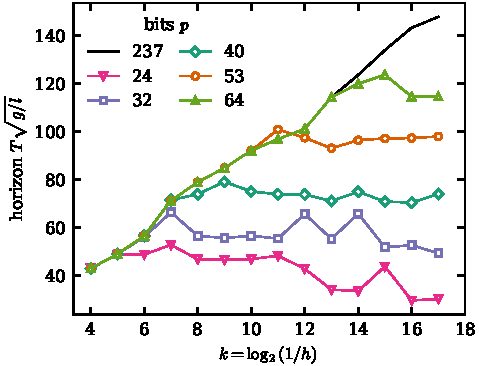
\includegraphics[width=\columnwidth]{fig5_turnover}
\caption{Horizon against step for five working precisions, with the 237-bit
result of Fig.~\ref{fig:hor}(a) for comparison. For each precision there is a
step beyond which further refinement does not help.}
\label{fig:turn}
\end{figure}

\begin{table}
\caption{Longest horizon attainable with RK4 at each precision, and the step at
which it occurs. The last column is for rods of length 1~m.}
\label{tab:best}
\begin{ruledtabular}
\begin{tabular}{lccc}
Significand bits $p$ & Best step & $T_{\max}\sqrt{g/l}$ & $T_{\max}$ (s) \\
\hline
\bestRows
\end{tabular}
\end{ruledtabular}
\end{table}

In double precision the horizon is about \TBestDouble\ time units, or
\TBestDoubleSec~s for a pendulum with one-meter rods, and it is reached at
$h=2^{-\kBestDouble}$. A student who responds to a doubtful result by reducing
the step to $2^{-17}$ does \kRatio\ times the work and gains nothing: the horizon
is \TdoubleFine. In single precision the horizon is \TBestSingle\ time units,
reached already at $h=2^{-\kBestSingle}$, and by $h=2^{-17}$ it has fallen to
\TsingleFine.

\subsection{Energy}
\label{sec:energy}

Figure~\ref{fig:energy} compares the two errors for an ordinary double-precision
run at $h=2^{-10}$. The error in the energy grows slowly, through the secular
drift of a non-symplectic method, and at the end of the run is still below
$10^{-\dEexp}$. The error in the position reaches the size of the apparatus at
$t\approx\TdoubleKten$. The reason is geometric. Energy constrains the state
to a three-dimensional surface in the four-dimensional phase space, and the
divergence of nearby trajectories takes place within that surface. A computed
state can drift an arbitrary distance along it without leaving it.

\begin{figure}
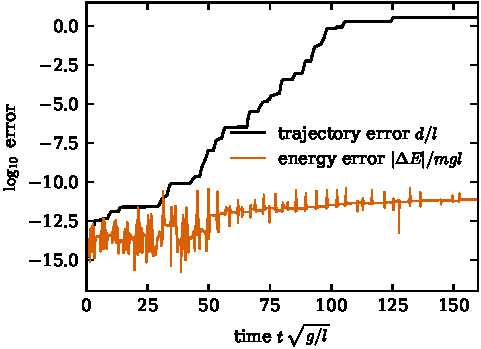
\includegraphics[width=\columnwidth]{fig6_energy}
\caption{Error in the position of the lower bob and error in the energy for one
run in double precision ($p=53$) with $h=2^{-10}$. Energy remains conserved to
better than a part in $10^{\dEexp}$ throughout, while the trajectory is lost near
$t=\TdoubleKten$.}
\label{fig:energy}
\end{figure}

\section{Discussion}

\subsection{What accuracy costs}

The work of a fixed-step integration is proportional to $2^{k}$. By
Eq.~(\ref{eq:Tk}), extending the horizon by $\Delta T$ requires
$\Delta k=\lambda\,\Delta T/(4\ln2)$, so the work is multiplied by
$e^{\lambda\Delta T/4}$; to stay on the optimum of Eq.~(\ref{eq:Tmax}) the
precision must rise as well, by about $\lambda\,\Delta T\,(4+\gamma)/(4\ln2)$
bits. For this pendulum, doubling the horizon attainable in double precision
multiplies the number of steps by roughly $e^{\lambda T_{\max}/4}\approx\costFactor$
and calls for some \extraBits\ additional bits. The horizon grows as the logarithm
of the effort spent on it. A method of order $n$ replaces the 4 by $n$, which is
the real argument for high-order integrators in this setting. We checked the low
end. At a fixed early time the error of forward Euler scales as $h^{\ordEuler}$,
that of the explicit midpoint rule as $h^{\ordMid}$, and that of RK4 as
$h^{\rkOrder}$, and the horizons lengthen in proportion: forward Euler with
$h=2^{-16}$ is accurate for \TEulerFine\ time units, which is less than the
\TRKcoarse\ that RK4 achieves with $h=2^{-4}$ and a thousandth of the work.

In everyday units the result is easy to remember. For rods one meter long
$\lambda=\lamSI~\mathrm{s^{-1}}$, so reducing the step tenfold buys
$4\ln10/\lambda\approx\decadeSI$~s of accurate motion, at ten times the cost.

\subsection{What is still right after the horizon}

Beyond $T$ the computed trajectory is not the solution of the initial-value
problem that was posed. It is not meaningless, however. Shadowing
results\cite{hammel1987,hammel1988,grebogi1990,sauer1997} show that, for long
times, a noisy computed orbit of a chaotic system stays close to \emph{some} exact
orbit with a slightly different initial condition. Quantities that are
properties of the ensemble of orbits rather than of a particular one, such as
the Lyapunov exponent, are therefore computed correctly by runs hundreds of
horizons long. The first row of Table~\ref{tab:lambda} is such a computation, done
in double precision. The distinction between predicting a trajectory and sampling
the dynamics is the right note on which to leave a class.

\subsection{Use in a course}

The exercise suits a course in computational physics, classical mechanics or
numerical analysis at the upper-division level, after students have met RK4 and
floating-point numbers. The program is short, since the integrator is the usual
one with the number type changed, and every run in this paper completes in
minutes on a laptop except the two finest references. Students who have only
hardware arithmetic can still do the third experiment, using a double-precision
run at the best step of Table~\ref{tab:best} as the reference for single
precision. The original version of this project was carried out in exactly that
spirit, with decimal steps and a handful of precisions, and the logarithmic law
was evident even there: each tenfold reduction of the step bought between five
and ten seconds.

\section{Suggested problems}

\begin{enumerate}
\item \emph{Order of the method.} Replace RK4 with forward Euler and with the
midpoint rule, repeat the first experiment, and show that the slope of $T$
against $k$ is $n\ln2/\lambda$ for a method of order $n$. Estimate the step that
Euler's method would need to match RK4 at $h=2^{-10}$.
\item \emph{Energy dependence.} Release the pendulum from rest at smaller angles.
Show that $\lambda$ decreases and the horizon lengthens, and that for
sufficiently small angles the error grows as a power of $t$ rather than
exponentially. What does Eq.~(\ref{eq:horizon}) become in that case?
\item \emph{The roundoff exponent.} Repeat the second experiment at several
steps and determine $\gamma$. Then replace the update
$\bm y\leftarrow\bm y+\Delta\bm y$ by compensated summation\cite{higham2002} and
determine it again.
\item \emph{A symplectic method.} Integrate with the implicit midpoint rule,
which is symplectic. Show that the energy error no longer drifts, and compare the
horizon with that of the explicit midpoint rule at the same step. Does
preserving the geometry of phase space help with predicting the trajectory?
\item \emph{Another system.} Carry out the first and third experiments for the
Lorenz equations with the standard parameters, for which
$\lambda\approx0.906$, and predict the double-precision horizon before measuring
it.
\item \emph{Shadowing.} Compute the time average of the kinetic energy over
$10^4$ time units in single and in double precision with $h=2^{-7}$. We find
1.357 and 1.358 in units of $mgl$. Explain why the two agree to a part in a
thousand although the trajectories separate after fifty time units.
\end{enumerate}

\ifanon
\else
\begin{acknowledgments}
This work began as a final project in Math~165, Numerical Analysis, at Harvey
Mudd College.
\end{acknowledgments}
\fi

\section*{Supplementary material}
The supplementary material contains the Python source for every computation and
figure in this paper, the numerical values plotted, and two animations: pendulums
differing only in step size, and pendulums differing only in precision, each
drawn beside its growing error.

\section*{Author declarations}
The authors have no conflicts to disclose.

\bibliography{../refs}

\end{document}
